%Beamer-Vorlage, v1.02

\documentclass{beamer}
\usepackage[T1]{fontenc}
\usepackage[utf8]{inputenc}
\usepackage[german]{babel}
\usepackage{graphicx}
\usepackage[osf]{libertine}
\usepackage{microtype}
\usepackage{booktabs}
\usepackage{nicefrac}
\usepackage{multirow}
\usepackage{csquotes}
\usepackage[loadonly]{enumitem}
\newlist{arrowlist}{itemize}{1}
\setlist[arrowlist]{label=$\Rightarrow$}

\usetheme{Madrid} %dieser Wert stellt das generelle Thema der Präsentation ein: Einfach einen der folgenden Namen eintragen
%Themes ohne Navigationsleiste: Boadilla, Pittsburgh, Rochester, Madrid, AnnArbor
%Themes mit baumartiger Navigationsleiste: Antibes, JuanLesPins, Montepellier
%Themes mit Inhaltsverzeichnis auf jeder Seite: Berkley, PaloAlto, Goettingen, Marburg, Hannover
%Themes mit Mini-Frame-Navigation: Berlin, Ilmenau, Dresden, Darmstadt, Frankfurth, Singapore, Szeged
%Themes mit Abschnitt/Unterabschnitt-Gliederung: Copenhagen, Luebeck, Malmoe, Warsaw

%\useinnertheme{default}
%default, circles, rectangels, rounded, inmargin

%\useoutertheme{default}
%default, infolines, miniframe, smoothbars, sidebar, split, shadow, tree, smouthtree

\usecolortheme[RGB={36,110,188}]{structure} %mit dieser Zeile kann man eigene Farbstile vorgeben, oder man verwendet eine der Namen aus den drei folgenden Zeilen (die Farben sind aber eher gruselig als brauchbar!)
%vollstaendig: default, arbatross, beetle, crane, dove, fly, seagull, wolverine
%inner color theme: lilly, orchid, rose
%outer color theme: whale, seahorse, dolphin

\setbeamerfont{frametitle}{size=\normalsize} %Dieser Werk setzt die Schriftgröße des Framtitle fest (Standard ist etwas größer)
\setbeamertemplate{navigation symbols}{}
\graphicspath{{img/}}

\title{Prävalenzabhägige Kontaktraten}

\date{14. Februar 2022} %wenn man hier "\today" einträgt, bekommt man das aktuelle Datum
\author{Mansur Daschaew, Janina Rastetter und Maren Raus}


\begin{document}
\maketitle

\tableofcontents

\section{Fallbeispiel Xi'an}
\begin{frame}
	\frametitle{Kontext und Begründung der Auswahl}
	China...
	\begin{itemize}
		\item strikte Null-Covid-Strategie in der Coronapandemie\only<2->{\\$\Rightarrow$ aktuelles Beispiel: Lockdown in der chinesischen Stadt Xi'an}\only<3->{\\ $\Rightarrow$ reale Daten}
		\only<1>{	
			\begin{center}
				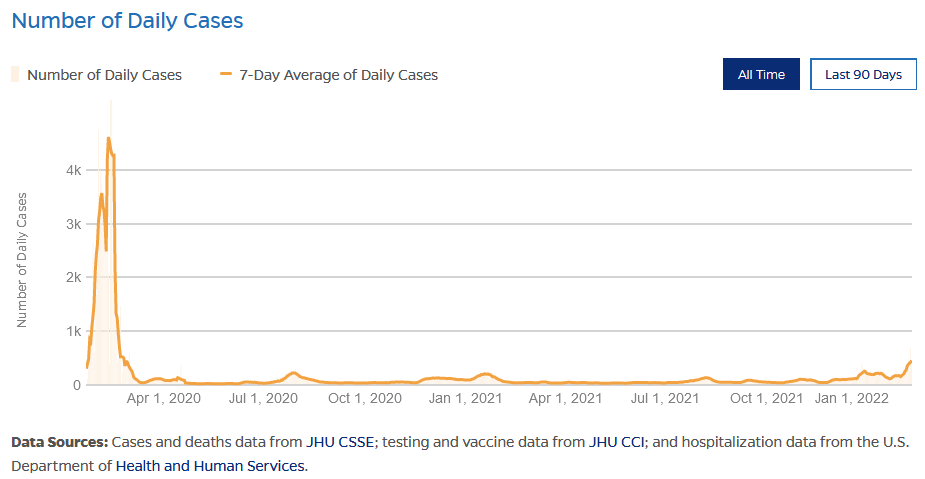
\includegraphics[scale=0.4]{john-hopkins-china.png}
			\end{center}}
		\only<2>{	
			\begin{center}
				
\includegraphics[scale=0.35]{spiegel-schlagzeile.png}
			\end{center}}
		\item <4->Impfquote von 87.88\%, aber bei verwendeter Vakzine kaum Schutz vor Delta\\$\Rightarrow$ Annahme: nicht immunisierte Bevölkerung 

	\end{itemize}
\end{frame}

\subsection{Vorgehen}
\begin{frame}
	\frametitle{Vorgehen}
	\begin{enumerate}
		\item Recherche (Daten zur Infektionslage in Xi'an und zur Deltavariante)
		\item Berechnung der Parameter
		\item Schätzung des Parameters $\delta$ (verantwortlich für die Identifikation infizierter Individuen)
		\item Berechnung der Anfangswerte
		\item Simulation verschiedener Szenerien mit dem Ziel, die Epidemie möglichst schnell ohne Durchseuchung stoppen
	\end{enumerate}
\end{frame}

\subsection{Daten}
\begin{frame}
	\frametitle{Daten}
	Dünne Datenlage
	\begin{itemize}
		\item 9. Dezember 2021: erster Fall
		\item In den Folgetagen: steigende Infektionszahlen
		\item 22. Dezember 2021 (+ 13 Tage): 63 Fälle
		\item 23. Dezember 2021: Lockdown
		\item 28. Dezember 2021 (+ 19 Tage): 175 Fälle
		\item 24. Januar 2022: Ende des Lockdowns (nach 32 Tagen), insgesamt ca. 2000 Fälle
	\end{itemize}
\end{frame}

\subsection{Parameter}
\begin{frame}
	\frametitle{Parameter}
	\begin{itemize}
		\item R-Wert $\approx 5.5$
		\item $\alpha = \nicefrac{1}{2}$ (mittlere Latzenzeit $\approx 4$, ansteckend etwa zwei Tag vor Auftreten von Symptomen)
		\item $\gamma = \nicefrac{1}{12}$
		\item $\beta \approx \gamma \cdot R = \nicefrac{5.5}{12} = 0.468$
		\item $\phi \approx \nicefrac{\gamma}{\beta} = \nicefrac{1}{5.5} $
		\item $\beta \cdot \phi = \nicefrac{1}{12}$
	\end{itemize}
\end{frame}

\subsection{Schätzung von $\delta$}
\begin{frame}
	\frametitle{Schätzung von $\delta$}
	Beobachtung: Schlechter Fit mit recherchierten Werten 
	\begin{center}
		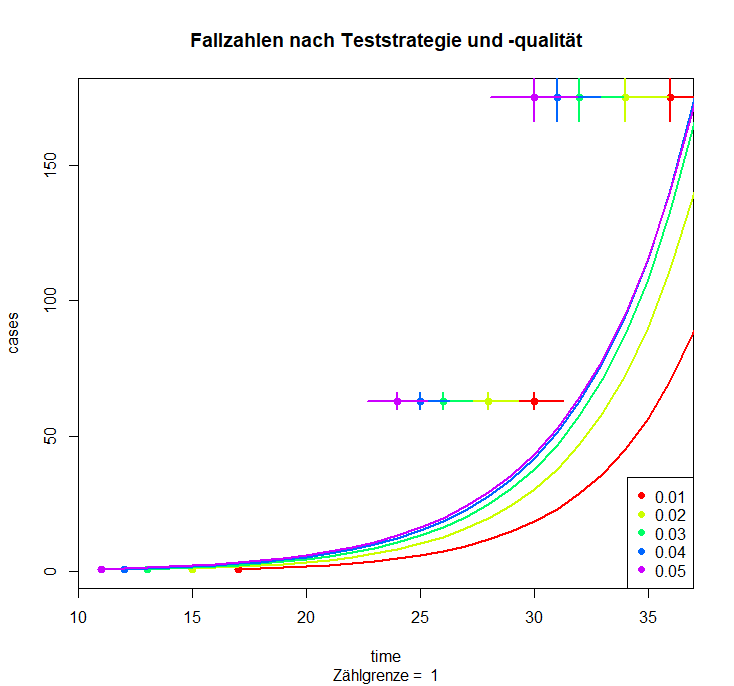
\includegraphics[scale=0.45]{delta_tol=1.png}
	\end{center}
\end{frame}

\begin{frame}
	\frametitle{Schätzung von $\delta$}
	Konsequenz: Erlaube Abweichungen $\Rightarrow \delta = 0.01$
	\begin{center}
		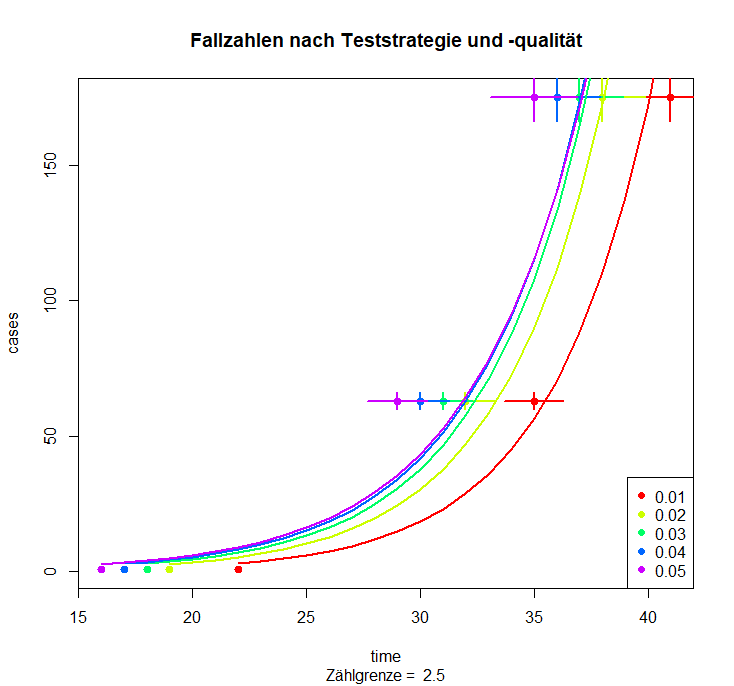
\includegraphics[scale=0.45]{delta_tol=2,5.png}
	\end{center}
\end{frame}

\subsection{Anfangswerte}
\begin{frame}
	\frametitle{Anfangswerte (gerundet)}
	\begin{itemize}
		\item $t = 36$
		\item $S = 12 996 450$
		\item $E = 1097$
		\item $I = 1731$
		\item $C = 56$
		\item $R = 666$		
	\end{itemize}
\end{frame}

\subsection{Simulationen}
\begin{frame}
	\frametitle{Verlauf ohne Intervention}
	\begin{center}
		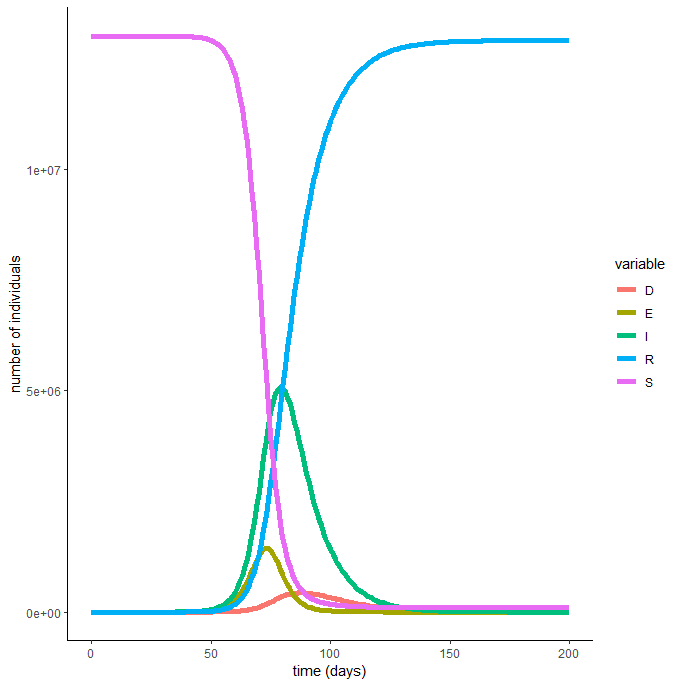
\includegraphics[scale=0.45]{delta=0,01,beta_unveraendert,alles.png}
	\end{center}
\end{frame}

\begin{frame}
	\frametitle{Verlauf ohne Intervention}
	\begin{table}[h]
		\caption{Verlauf ohne Intervention}
		\centering
		\begin{tabular}{@{}ccc@{}}
			\toprule
			Kompartment & Maximum & Zeitpunkt des Maximums\\ 
			\midrule
			I &  5076922& 80\\ 
			E & 1437318 & 74\\ 
			D &  433135.2 & 89 \\ 
			\bottomrule
		\end{tabular}
	\end{table}
	\vspace{0.5cm}
	\begin{itemize}
		\item Verbleibende S: 99439.98 (0.7649229\%)\\	$\Rightarrow$ Durchseuchung
		\item Schritte, bis E und I kleiner 1: 260
	\end{itemize}
\end{frame}

\begin{frame}
	\frametitle{Erhöhung der Testungen}
	\begin{table}[h]
		\caption{Verlauf mit verstärktem Testen}
		\centering
		\begin{tabular}{@{}ccc@{}}
			\toprule
			$\delta$ & Verbleibende S (in \%) & I und E kleiner 1, ab\\ 
			\midrule
			 $\delta_{ur} \cdot 2^1$ & 1.252596 & 212 (+ 36) \\ 
			 $\delta_{ur} \cdot 2^2$ & 2.687945 & 196 (+ 36)\\  
			 $\delta_{ur} \cdot 2^3$ & 7.447852 & 186 (+ 36)\\ 
			 $\delta_{ur} \cdot 2^4$ & 23.80182 & 211 (+ 36)\\ 
			 $\delta_{ur} \cdot 2^5$ & 76.87228 & 589 (+ 36)\\ 
			 $\delta_{ur} \cdot 2^6$ & 99.93514 & 60 (+ 36)\\ 
			\bottomrule
		\end{tabular}
	\end{table}
	\vspace{0.5cm}
	\begin{arrowlist}
		\item Erst ab einer Steigerung der Testeffizienz um Faktor $2^5$ ist eine Eindämmung der Epidemie möglich
		\item Bei einer Steigerung der Testeffizienz um Faktor $2^6$ müssten \enquote{nur} zwei Monate lang vermehrt getestet werden
	\end{arrowlist}
\end{frame}

\begin{frame}
	\frametitle{Verlauf mit verstärktem Testen: $\delta = 0.64$}
	\begin{center}
		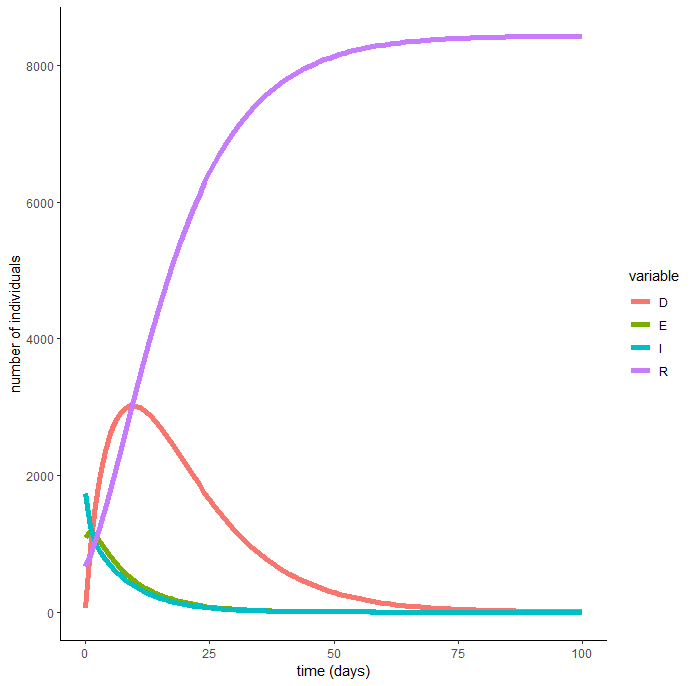
\includegraphics[scale=0.45]{delta=0,64,beta_unveraendert,ohne_s.png}
	\end{center}
\end{frame}

\begin{frame}
	\frametitle{Verlauf mit verstärktem Testen: $\delta = 0.64$}
	\begin{table}[h]
		\caption{Verlauf mit verstärktem Testen: $\delta = 0.64$}
		\centering
		\begin{tabular}{@{}ccc@{}}
			\toprule
			Kompartment & Maximum & Zeitpunkt des Maximums\\ 
			\midrule
			I & 1731 & 0\\ 
			E & 1185.318 & 1\\ 
			D & 3016.812 &  9\\ 
			\bottomrule
		\end{tabular}
	\end{table}
\end{frame}

\begin{frame}
	\frametitle{Reduktion der Kontakte}
		\begin{table}[h]
		\caption{Verlauf mit Kontaktreduktion}
		\centering
		\begin{tabular}{@{}ccc@{}}
			\toprule
			$\beta$ & Verbleibende S (in \%) & I und E kleiner 1, ab\\ 
			\midrule
			$\beta_{ur} * 2^{-1}$ & 11.3365 & 338 (+ 36) \\ 
			$\beta_{ur} * 2^{-2}$  & 65.28979 &  1184 (+ 36)\\  
			\nicefrac{1}{12} & 99.79345 & 898 (+ 36)\\ 
			\bottomrule
		\end{tabular}
	\end{table}
	\begin{arrowlist}
		\item Kontaktreduktion verhindert Infektionen, zieht die Epidemie aber in die Länge
		\item Um eine Durchseuchung zu verhindern, müssten die Kontakte fast drei Jahre lang reduziert werden
	\end{arrowlist}
\end{frame}

\begin{frame}
	\frametitle{Verlauf mit Kontaktreduktion: $\beta = \nicefrac{1}{12}$}
	\begin{center}
		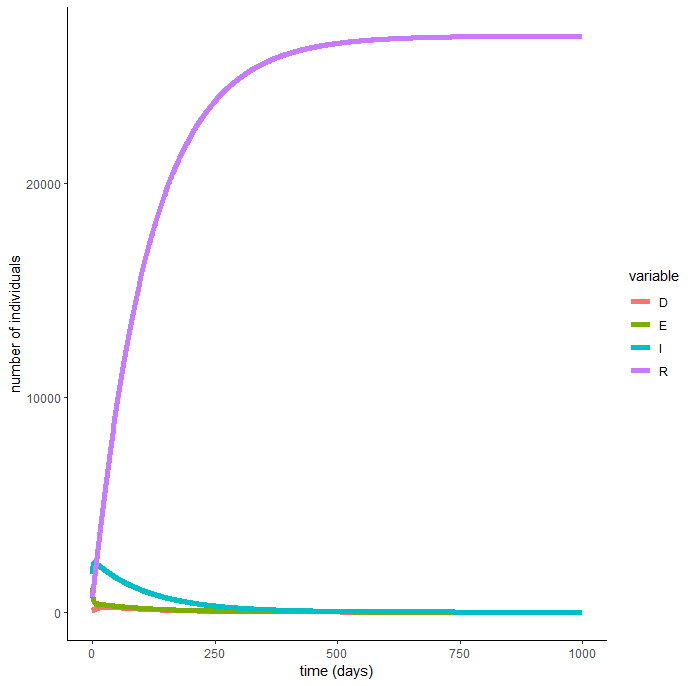
\includegraphics[scale=0.45]{delta=0,01,beta=1durch12,ohne_s.png}
	\end{center}
\end{frame}
%\begin{frame}
%	\frametitle{Verlauf mit Kontaktreduktion: $\beta = \beta_{ur} * 2^{-3}$}
%	\begin{center}
%		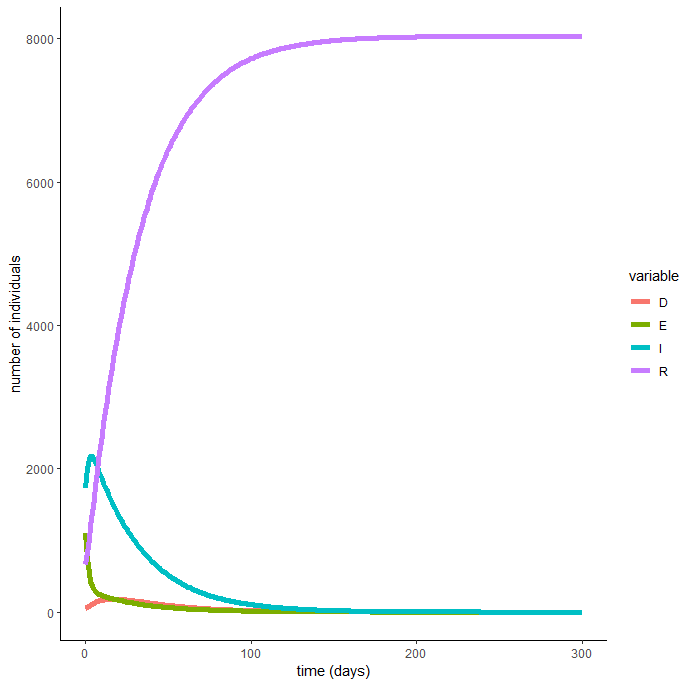
\includegraphics[scale=0.45]{delta=0,01,beta=0,125beta,ohne_s.png}
%	\end{center}
%\end{frame}

\begin{frame}
	\frametitle{Verlauf mit Kontaktreduktion: $\beta = \nicefrac{1}{12}$}
	\begin{table}[h]
		\caption{Verlauf mit Kontaktreduktion: $\beta = \nicefrac{1}{12}$}
		\centering
		\begin{tabular}{@{}ccc@{}}
			\toprule
			Kompartment & Maximum & Zeitpunkt des Maximums\\ 
			\midrule
			I & 2288.959 & 5 (+36)\\ 
			E & 1097 & 0 (+36)\\ 
			D & 228.0604 &  29 (+36)\\ 
			\bottomrule
		\end{tabular}
	\end{table}
\end{frame}

\begin{frame}
	\frametitle{Erhöhung der Testungen und Kontaktreduktion: $\beta = \nicefrac{1}{12}$}
	\begin{table}[h]
		\caption{Verlauf mit verstärktem Testen und Kontaktreduktion}
		\centering
		\begin{tabular}{@{}ccc@{}}
			\toprule
			$\delta$ & Verbleibende S (in \%) & I und E kleiner 1, ab\\ 
			\midrule
			 %$\delta_{ur} \cdot 2^0$ & 99.79345 & 898 (+ 36)\\  
			 $\delta_{ur} \cdot 2^1$ & 99.88242 & 456 (+ 36) \\ 
			 $\delta_{ur} \cdot 2^2$ & 99.92746 & 230 (+ 36)\\  
			 $\delta_{ur} \cdot 2^3$ & 99.95006 & 117 (+ 36) \\ 
			 $\delta_{ur} \cdot 2^4$ & 99.96137 & 60 (+ 36)\\ 
			 $\delta_{ur} \cdot 2^5$ & 99.96703 & 33 (+ 36)\\ 
			 $\delta_{ur} \cdot 2^6$ & 99.96986 & 20 (+ 36)\\ 
			\bottomrule
		\end{tabular}
	\end{table}
	%\vspace{0.5cm}
	\begin{arrowlist}
		\item Bei extremer Kontaktreduktion wirkt sich die Testeffizienz kaum auf die Anzahl der Infektionen aus, dafür aber sehr stark auf die erforderliche Dauer der Beschränkungen
		\item Die Testeffizienz müsste mindestens um Faktor $2^4$ gesteigert werden, um die Dauer der Einschränkungen gering zu halten (ein bis zwei Monate)
	\end{arrowlist}
\end{frame}

\begin{frame}
	\frametitle{Verlauf mit Kontaktreduktion und verstärktem Testen: $\beta = \nicefrac{1}{12}$ und $\delta = 0.32$}
	\begin{center}
		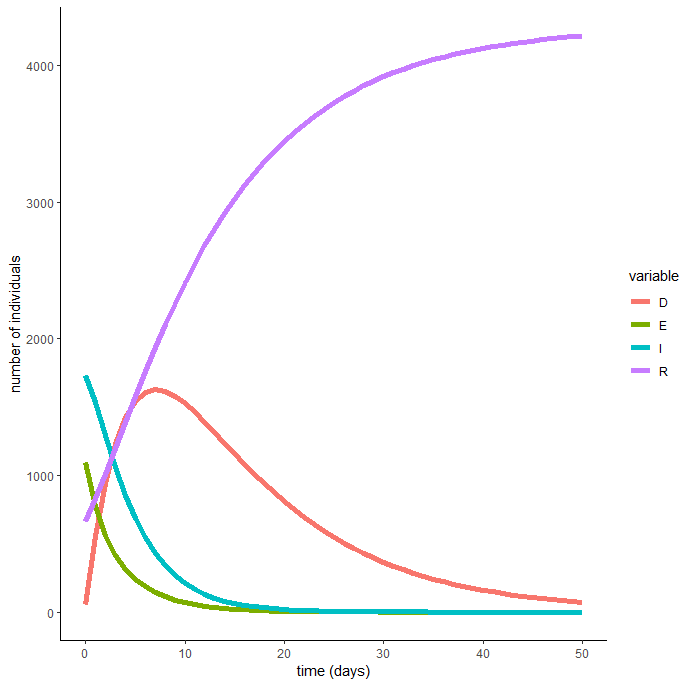
\includegraphics[scale=0.45]{delta=0,32,beta=1durch12,ohne_s.png}
	\end{center}
\end{frame}

\begin{frame}
	\frametitle{Verlauf mit Kontaktreduktion und verstärktem Testen: $\beta = \nicefrac{1}{12}, \delta = 0.32$}
	\begin{table}[h]
		\caption{Verlauf mit Kontaktreduktion und verstärktem Testen: $\beta = \nicefrac{1}{12}, \delta = 0.32$}
		\centering
		\begin{tabular}{@{}ccc@{}}
			\toprule
			Kompartment & Maximum & Zeitpunkt des Maximums\\ 
			\midrule
			I & 1731 & 0\\ 
			E & 1097 & 0\\ 
			D & 1627.685 & 7\\ 
			\bottomrule
		\end{tabular}
	\end{table}
\end{frame}

\begin{frame}
	\frametitle{Verlauf mit Kontaktreduktion und verstärktem Testen: $\beta = \nicefrac{1}{12}$ und $\delta = 0.64$}
	\begin{center}
		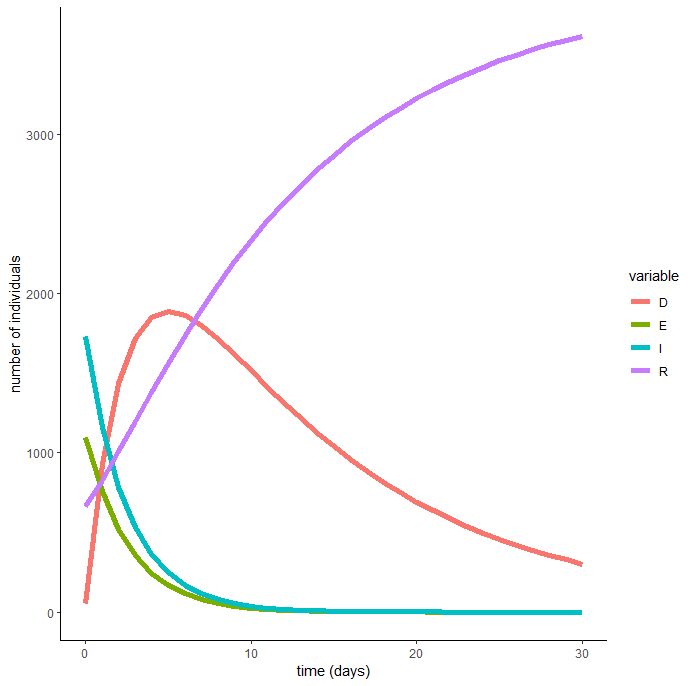
\includegraphics[scale=0.45]{delta=0,64,beta=1durch12,ohne_s.png}
	\end{center}
\end{frame}

\begin{frame}
	\frametitle{Verlauf mit Kontaktreduktion und verstärktem Testen: $\beta = \nicefrac{1}{12}, \delta = 0.64$}
	\begin{table}[h]
		\caption{Verlauf mit Kontaktreduktion und verstärktem Testen: $\beta = \nicefrac{1}{12}, \delta = 0.64$}
		\centering
		\begin{tabular}{@{}ccc@{}}
			\toprule
			Kompartment & Maximum & Zeitpunkt des Maximums\\ 
			\midrule
			I & 1731 & 0\\ 
			E & 1097 & 0\\ 
			D & 1886.614 &  5\\ 
			\bottomrule
		\end{tabular}
	\end{table}
\end{frame}

\begin{frame}
	\frametitle{Erhöhung der Testungen und Kontaktreduktion: $\delta = \nicefrac{1}{12}$}
	\begin{table}[h]
		\caption{Verlauf mit verstärktem Testen und Kontaktreduktion}
		\centering
		\begin{tabular}{@{}cc@{}}
			\toprule
			$\delta$ & Fälle (gesamt)\\ 
			\midrule
			 %$\delta_{ur} \cdot 2^0$ & 99.79345 & 898 (+ 36)\\  
			 $\delta_{ur} \cdot 2^1$ & 34473.27 (+ 348.5105)\\ 
			 $\delta_{ur} \cdot 2^2$ & 34566.07 (+ 348.5105)\\  
			 $\delta_{ur} \cdot 2^3$ & 34596.05 (+ 348.5105)\\ 
			 $\delta_{ur} \cdot 2^4$ & 34584.94 (+ 348.5105)\\ 
			 $\delta_{ur} \cdot 2^5$ & 33786.95 (+ 348.5105)\\ 
			 $\delta_{ur} \cdot 2^6$ & 31079.05 (+ 348.5105)\\ 
			\bottomrule
		\end{tabular}
	\end{table}
	%\vspace{0.5cm}
	\begin{arrowlist}
		\item Fehler bei Parameterwahl, in Xi'an gab es insgesamt nur etwa 2000 Fälle
		\item Vermutung zur Fehlerquelle:\\Lockdown in Xi'an bei $t=14$, in Simulation bei $t=36$\\Schätzung von $\delta$ darf sich nicht zu stark auf den Anfangszeitpunkt der Maßnahmen auswirken
	\end{arrowlist}
\end{frame}

\begin{frame}
	\frametitle{Zusammenfassung}
	\begin{table}[h]
		\caption{Zusammenfassung}
		\centering
		\begin{tabular}{@{}ccccc@{}}
			\toprule
			Strategie & $\delta$ & $\beta$ & Dauer & Verbleibende S (in \%)\\ 
			\midrule
			-- & 0.01 & \nicefrac{5.5}{12} & 8.5 Monate & 0.7649229\\
			T &  0.64 & \nicefrac{5.5}{12} & 2 Monate & 99.93514\\ 
			K & 0.01 & \nicefrac{1}{12} & 2.5 Jahre & 99.79345\\
			K + T & 0.32 & \nicefrac{1}{12} & 1 Monat & 99.96703\\
			K + T & 0.64 & \nicefrac{1}{12} & 3 Wochen & 99.96986\\
			\bottomrule
		\end{tabular}
	\end{table}
\end{frame}

%\begin{frame}
%	\frametitle{Was kostet ein Lockdown? -- Eine naive Rechnung}
%\end{frame}


%\part{Vorlesung 1} % mit "part" kann man seine Vorträge noch weiter gliedern, zum Beispiel für jede Vorlesung eine eigene mit jeweils eigenem Inhaltsverzeichnis und Struktur
%\section{Einleitung}
%
%\begin{frame}
%	\frametitle{Verbreitung der Schildkröten}
%	\begin{center}
%	%\includegraphics[width=0.7\textwidth]{Karte.png}
%	
%	{\small Die Weltkarte vor 400 Millionen Jahren. Links der Urkontinent, rechts seine Begleiter. Der Pfeil zeigt auf die Fundschicht der Schildkröten.}
%
%	\end{center}
%\end{frame}
%
%\section{Spezieller Teil}
%\subsection{Taxonomie}
%
%\begin{frame}
%	\frametitle{Schildkrötenarten}
%
%	Es gibt insgesamt 20 bekannte Gattungen paläozoischer Schildkröten, sie treten stratigrafisch wie folgt auf:
%	
%	\begin{block}{Gattungen} %erzeugt einen einfachen Block
%		\textit{Turtleiana brodeana}
%		
%		\textit{Comminsunia elegans}
%		
%		\textit{Joldia fingeri}
%		
%		\dots
%	\end{block}
%
%\end{frame}
%
%\subsection{Ontogenie}
%
%\begin{frame}
%	\frametitle{Wie Schildkröten heranwachsen}
%
%	Schildkröten sind Lebewesen, die durch viele Dinge beeinflusst werden, das sind zum Beispiel:
%	
%	\begin{exampleblock}{Dinge, die Schildis Heranwachsen beeinflussen} %Block für Beispiele
%		Luftfeuchtigkeit
%		
%		Tageszeit
%		
%		Stellung des Saturn im Sternbild Schütze
%	\end{exampleblock}
%
%\end{frame}
%
%\section{Zusammenfassung}
%
%\begin{frame}
%	\frametitle{Besonderheiten bei paläozoischen Schildkröten}
%	
%	\begin{itemize}
%		\item sind viel schwerfälliger
%		\item haben grüne Augen
%		\item jedes Weibchen wirft stets 3 Jungen
%	\end{itemize}
%	
%	\begin{alertblock}{Achtung!} %Block für Warnungen
%		Es gibt Ausnahmen!
%	\end{alertblock}
%\end{frame}
%
%\begin{frame}
%	\frametitle{Wie war das mit der Geografie?}
%	
%	\begin{columns} %benutze die Column-Umgebung, um Text und Bild oder Text und Text nebeneinander darzustellen
%		\column[c]{6cm} %erzeugt zentriert ausgerichtete Spalte mit 6 cm Breite
%		%	\includegraphics[height=3cm]{Karte.png}
%		\column{.45\textwidth} %erzeugt eine Spalte, die 45 % der Textbreite einnimmt
%			Kommen wir nochmal auf die Geografie zurück.
%	\end{columns}	
%\end{frame}
%
%\section{Ende}
%
%\begin{frame}
%	\frametitle{Ende}
%	\begin{center}
%	Danke für die Aufmerksamkeit! -- Fragen? \vspace{0.3cm}
%
%	
%	{\footnotesize www.schildis.de}
%	\end{center}
%\end{frame}

\end{document}